\documentclass[conference]{IEEEtran}

\usepackage[utf8]{inputenc}
\usepackage[T1]{fontenc}
\usepackage[spanish,es-nodecimaldot]{babel}
\usepackage{amsmath,amssymb}
\usepackage{graphicx}
\usepackage{booktabs}
\usepackage{siunitx}
\usepackage{microtype}
\usepackage{balance}
\usepackage{placeins}
\usepackage{eso-pic}
\usepackage{stfloats}

\sisetup{output-decimal-marker={,},per-mode=symbol}
\graphicspath{{figuras/}{../../05_Resultados/figuras/}{../../05_Resultados/Seleccion_Referencia/}}

\title{Laboratorio 9: Control óptimo digital con acción integral}

\author{\IEEEauthorblockN{Aldo Pastore}
\IEEEauthorblockA{Automatización -- Ingeniería Electrónica\\
Facultad de Ciencias y Tecnología\\
Universidad Católica “Nuestra Señora de la Asunción”\\
Asunción, Paraguay\\
\texttt{aldo.pastore@uc.edu.py}}}

\begin{document}
\maketitle

\begin{abstract}
Se diseñaron e implementaron tres reguladores LQR digitales con acción integral para una planta analógica de segundo orden. El controlador y el estimador se obtuvieron directamente del modelo identificado, con un período de muestreo de \SI{2}{ms}. Antes de ensayar el lazo se evaluaron referencias entre 0,25 y \SI{1}{V}; se seleccionó \SI{0.5}{V} porque utiliza una fracción apreciable del rango de la planta y mantiene el mando solicitado por debajo de \SI{0.8}{V}. Las respuestas se capturaron físicamente con un osciloscopio RIGOL, midiendo en forma simultánea el mando en J5 y la salida en J7. Los tiempos de subida medidos fueron 146, 16 y \SI{46}{ms} para los casos 1, 2 y 3. El caso 2 resultó el más rápido y demandó el intervalo de mando más amplio, de $-223$ a \SI{681}{mV}. Ningún controlador alcanzó el límite de actuación, aunque el error final medido quedó entre 15,8 y \SI{20.0}{mV}. El proyecto se compiló y programó desde PSoC Creator 4.4 y, al finalizar, la placa quedó nuevamente en modo seguro \texttt{MONITOR}.
\end{abstract}

\begin{IEEEkeywords}
acción integral, control digital, estimador de estados, LQR, modelo identificado, PSoC 5LP.
\end{IEEEkeywords}

\section{Introducción}
La realimentación de estados permite fijar una dinámica estable, pero no establece por sí sola un compromiso entre rapidez y esfuerzo de control. El regulador cuadrático lineal incorpora ese compromiso mediante un índice de costo. Al ampliar el sistema con la integral del error, también se obtiene seguimiento de referencias constantes frente a pequeñas diferencias de ganancia \cite{ogata,franklin}.

El objetivo fue comparar tres ponderaciones LQR, implementar un estimador actual y verificar el funcionamiento completo sobre la planta. El diseño se realizó con el modelo identificado, ya que es la representación que describe mejor el montaje. El modelo calculado a partir de los componentes se conservó únicamente para examinar sensibilidad.

\section{Modelo y discretización}
El modelo identificado tiene ganancia $K=1.002941$ y constantes de tiempo $\tau_1=\SI{9.06915}{ms}$ y $\tau_2=\SI{0.774399}{ms}$. Con estados compatibles con las tensiones internas, discretización ZOH y $T_s=\SI{2}{ms}$:
\begin{align}
x[k+1]&=A_{id}x[k]+B_{id}u[k], & y[k]&=Cx[k],\\
A_{id}&=\begin{bmatrix}0.802095&0\\-0.249628&0.075574\end{bmatrix},\\
B_{id}&=\begin{bmatrix}-0.631611\\0.130459\end{bmatrix},&
C&=\begin{bmatrix}0&1\end{bmatrix}.
\end{align}
Se obtuvo $\operatorname{rank}\mathcal{C}(A_{id},B_{id})=2$ y $\operatorname{rank}\mathcal{O}(A_{id},C)=2$. El sistema es, por tanto, controlable y observable.

El muestreo se verificó sobre la dinámica cerrada más rápida. El par dominante del caso 2, $0.6633\pm j0.2006$, equivale a $s=-183.4\pm j146.9\ \mathrm{rad/s}$ y $\omega_n=\SI{234.9}{rad/s}$. Como $\omega_s=2\pi/T_s=\SI{3141.6}{rad/s}$, resulta $\omega_s/\omega_n=13.37>10$. Además, el menor tiempo de subida simulado, \SI{12}{ms}, contiene seis períodos de muestreo. Por tanto, $T_s=\SI{2}{ms}$ permite representar la dinámica prevista con margen y coincide con el período validado en el montaje.

El estado integral se definió como
\begin{equation}
\xi[k+1]=\xi[k]+r[k]-y[k],
\end{equation}
de donde
\begin{equation}
A_a=\begin{bmatrix}A_{id}&0\\-C&1\end{bmatrix},\qquad
B_a=\begin{bmatrix}B_{id}\\0\end{bmatrix}.
\end{equation}
La matriz de controlabilidad de $(A_a,B_a)$ tiene rango 3. La ley implementada fue
\begin{equation}
u[k]=-K_x\hat{x}[k]-K_i\xi[k].
\end{equation}

\begin{table}[!t]
\caption{Ponderaciones y ganancias LQR}
\label{tab:ganancias}
\centering
\scriptsize
\setlength{\tabcolsep}{3.5pt}
\begin{tabular}{cccccc}
\toprule
Caso & $\operatorname{diag}(Q_1)$ & $Q_2$ & $K_x$ & $K_i$ & $\rho(A_{cl})$\\
\midrule
1 & $[.01,.01,.001]$ & 1 & $[-.05296,\ .03363]$ & $-.03099$ & .9701\\
2 & $[.01,.01,.1]$ & .1 & $[-.57981,\ .83718]$ & $-.77384$ & .6930\\
3 & $[.01,.01,.001]$ & .01 & $[-.60812,\ .25768]$ & $-.23297$ & .9125\\
\bottomrule
\end{tabular}
\end{table}

Los polos de lazo cerrado fueron $\{0.0756,0.7941,0.9701\}$, $\{0.0756,0.6633\pm j0.2006\}$ y $\{0.0766,0.4709,0.9125\}$ para los casos 1, 2 y 3. Sus radios espectrales explican el orden de rapidez previsto. La ecuación de Riccati convergió en 395, 39 y 129 iteraciones; se detuvo cuando $\|S_{k+1}-S_k\|_\infty<10^{-12}$ y se verificó con \texttt{dlqr}. La mayor diferencia entre ambas soluciones fue $3.35\times10^{-11}$.

\section{Estimador e implementación digital}
La salida estimada se calcula a partir del estado predicho y luego se compara con la salida medida. La secuencia utilizada en cada muestra es
\begin{align}
\hat{x}^{-}[k]&=A_{id}\hat{x}[k-1]+B_{id}u_{ap}[k-1],\\
\hat{y}^{-}[k]&=C\hat{x}^{-}[k],\\
\nu[k]&=y[k]-\hat{y}^{-}[k],\\
\hat{x}[k]&=\hat{x}^{-}[k]+L\nu[k].
\end{align}
Para polos del estimador en $0.20\pm j0.10$ se obtuvo
\begin{equation}
L=\begin{bmatrix}-1.860494424&0.175152235\end{bmatrix}^{T}.
\end{equation}
Así, $\nu[k]$ representa la diferencia entre la medición y la salida reconstruida a partir de los estados estimados.

\begin{figure*}[!t]
\centering
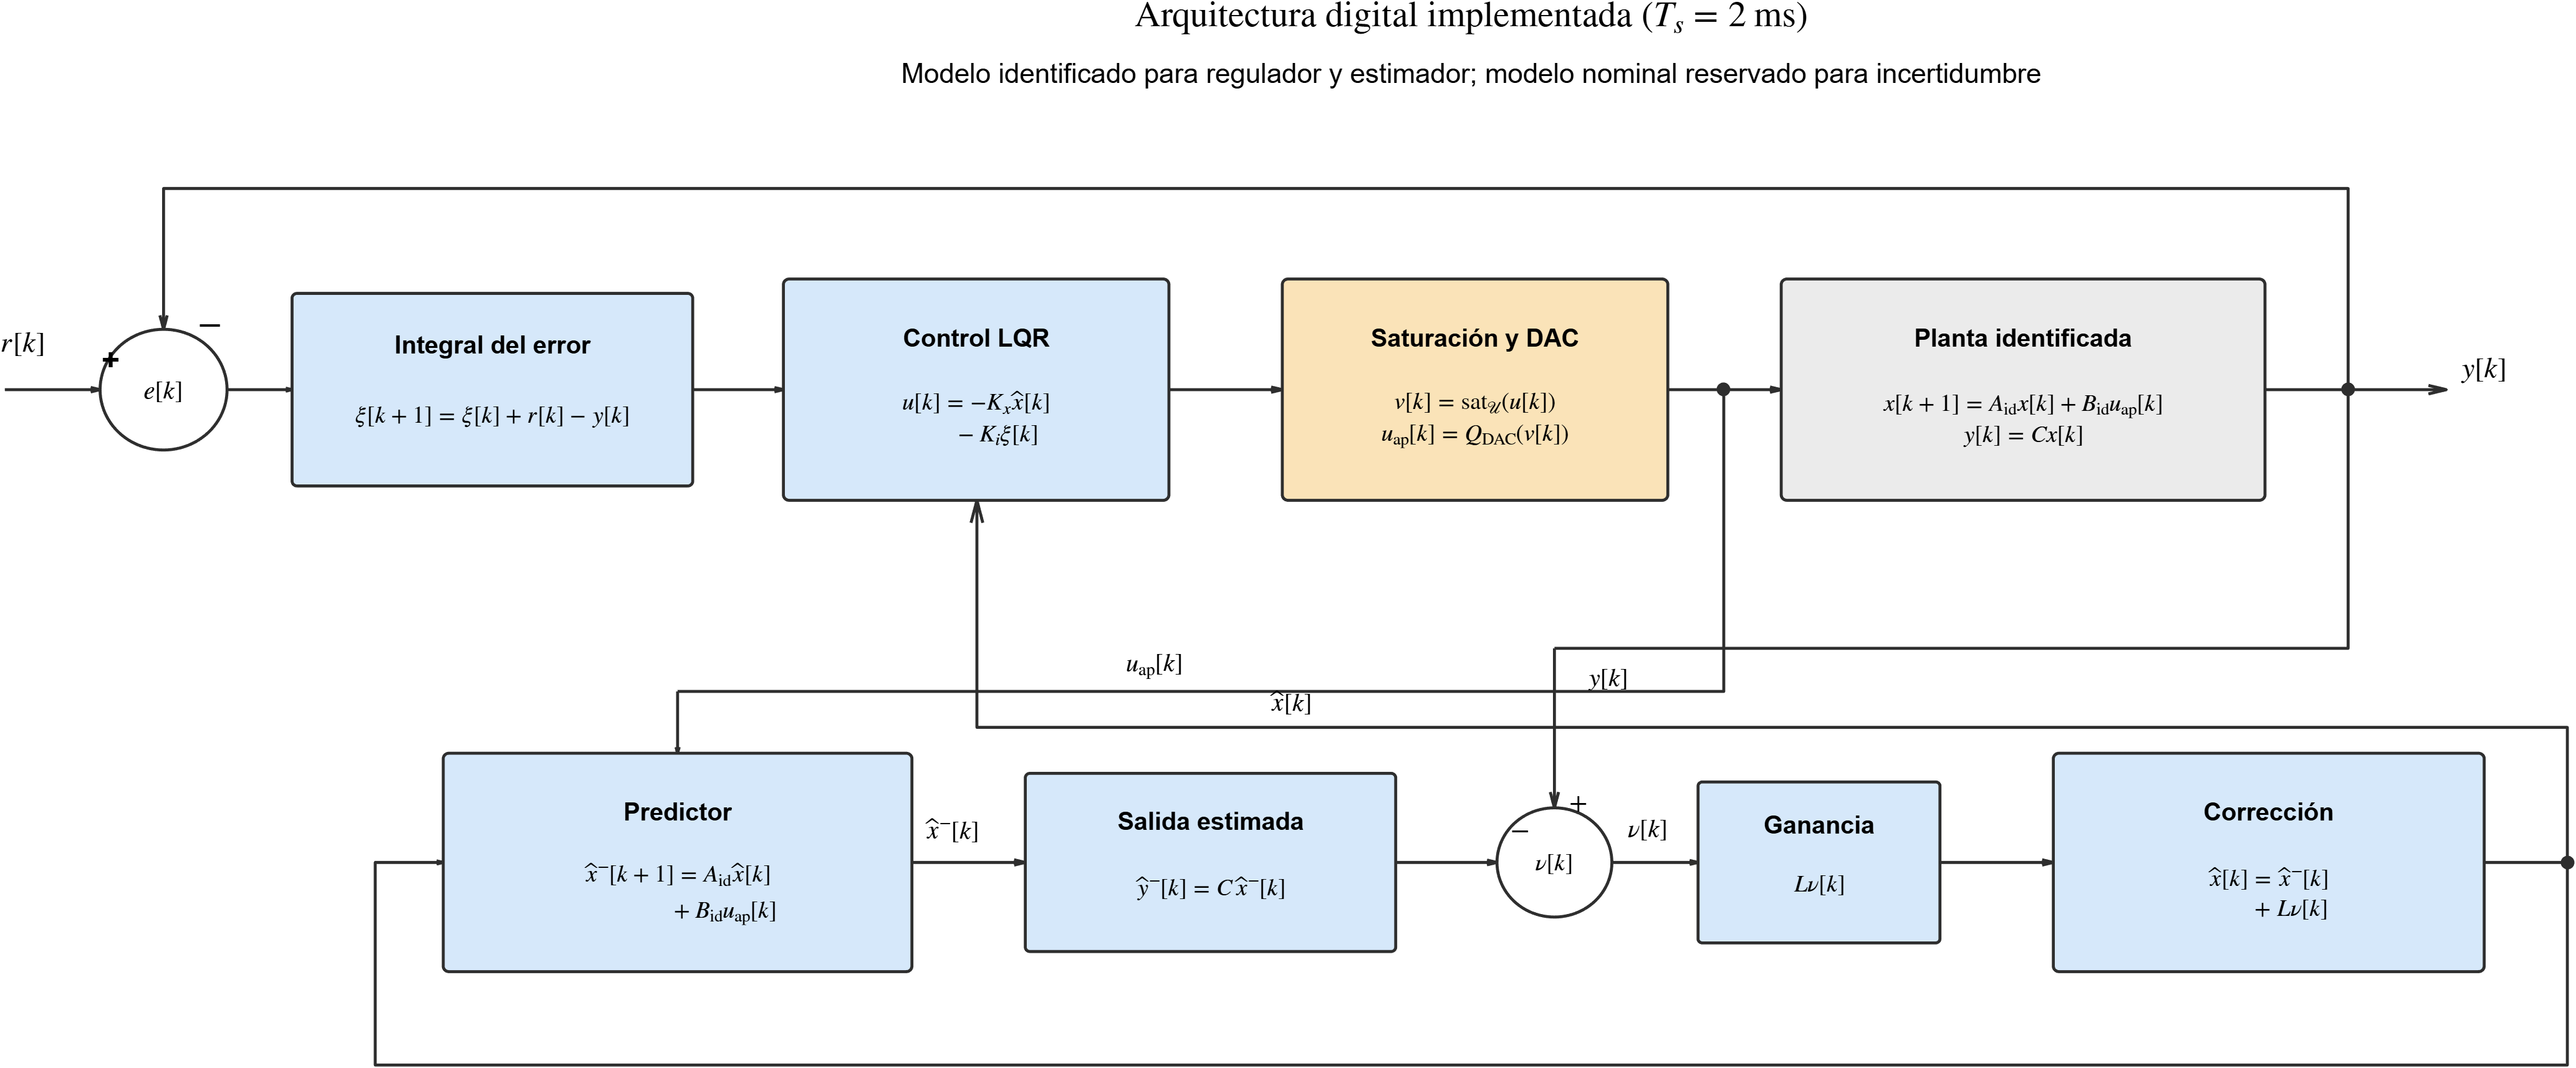
\includegraphics[width=0.96\textwidth]{diagrama_bloques_lab9.png}
\caption{Arquitectura digital implementada y realización en bloques de la planta identificada. La salida estimada $\hat y^{-}$ se obtiene de $\hat x^{-}$ y se resta de la salida medida para formar la innovación $\nu$. Los puntos negros indican bifurcaciones; los cruces sin punto no representan conexión.}
\label{fig:diagrama}
\end{figure*}

El firmware ejecuta adquisición, corrección del estimador, cálculo del control, saturación y actualización del predictor dentro de una interrupción periódica. El mando se limita a $\pm\SI{1}{V}$ y se convierte mediante dos DAC unipolares. También se incorporaron anti-windup, comprobaciones de rango, parada segura y enclavamientos de compilación. El código entregado queda en \texttt{MONITOR}, con ambos DAC en cero y las autorizaciones de actuación deshabilitadas.

\section{Selección de la referencia}
Para fijar la amplitud del ensayo se simularon 0,25, 0,50, 0,75 y \SI{1.00}{V} con los tres controladores y el modelo identificado. Se exigió ausencia de saturación y $|u|_{\max}\leq\SI{0.8}{V}$, dejando un margen de \SI{0.2}{V} respecto del límite físico.

\begin{table}[!t]
\caption{Barrido previo de amplitud}
\label{tab:amplitud}
\centering
\small
\begin{tabular}{cccc}
\toprule
$r$ [V] & peor $|u|$ [V] & saturaciones & criterio\\
\midrule
0,25 & 0,343 & 0 & cumple\\
0,50 & 0,687 & 0 & seleccionado\\
0,75 & 1,010 & 1 & no cumple\\
1,00 & 1,180 & 11 & no cumple\\
\bottomrule
\end{tabular}
\end{table}

La referencia de \SI{0.5}{V} fue la mayor que cumplió el criterio para los tres diseños. En el osciloscopio corresponde a unas 2,5 divisiones con la escala de \SI{0.2}{V/div} utilizada en el ensayo, y todavía conserva margen para incertidumbres y perturbaciones.

\begin{figure}[!t]
\centering
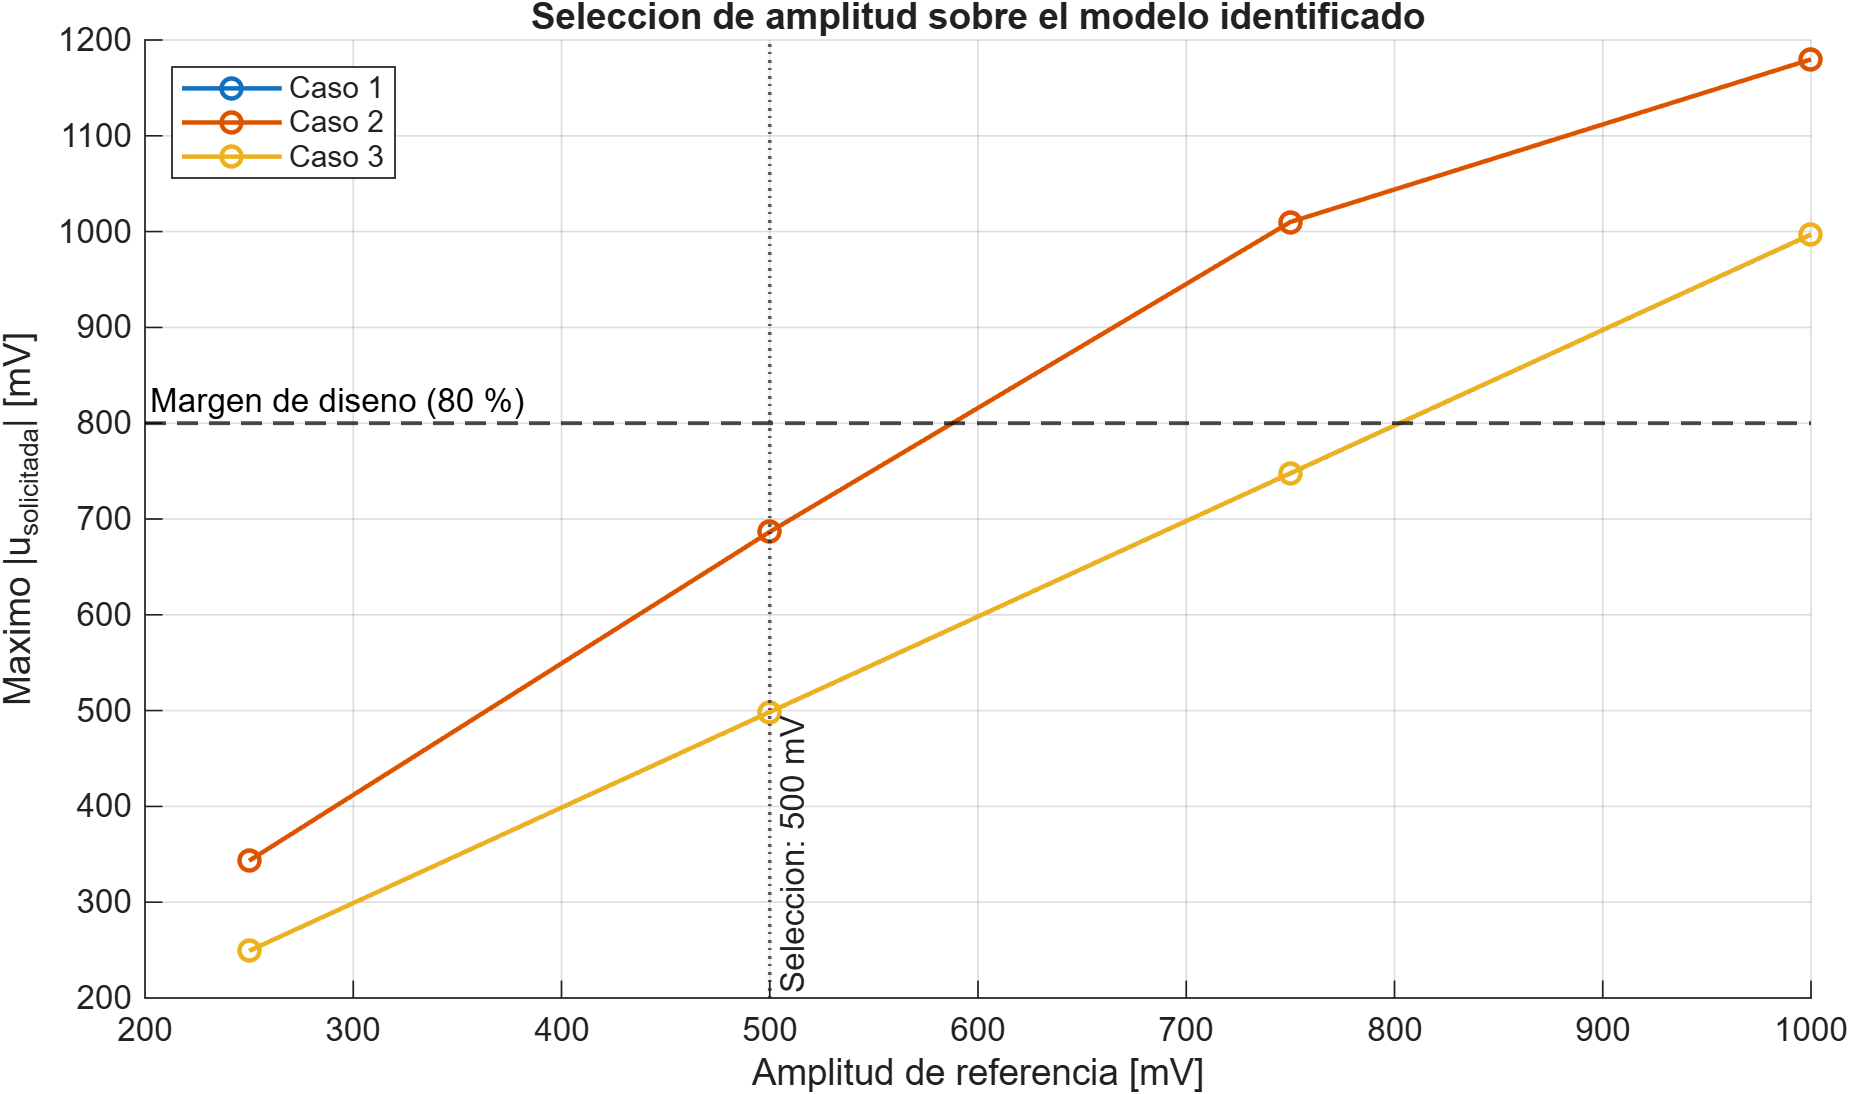
\includegraphics[width=\columnwidth]{seleccion_referencia_lab9.png}
\caption{Máximo esfuerzo solicitado durante el barrido de amplitud.}
\label{fig:seleccion}
\end{figure}

\section{Simulación}
Se simularon el actuador ideal limitado y el actuador con escalas reales de DAC. Para la rama positiva se emplearon \SI{15.370448}{mV} por código y para la negativa \SI{10.560423}{mV} por código. Ninguno de los tres casos saturó con \SI{0.5}{V}.

En la planta identificada con DAC cuantizado, los tiempos de subida fueron 148, 12 y \SI{48}{ms}; los tiempos de establecimiento al 2\,\% fueron 248, 18 y \SI{90}{ms}. El mayor sobreimpulso simulado fue 1,84\,\% en el caso 2. Los extremos de mando fueron \SIrange{0}{507}{mV}, \SIrange{-190}{692}{mV} y \SIrange{0}{507}{mV}.

Como verificación independiente, el modelo equivalente en Simulink reprodujo los extremos de mando calculados en MATLAB con diferencias menores que \SI{1}{\micro V}.

\noindent\begin{minipage}{\columnwidth}
Al aplicar las ganancias a la planta nominal, los tres lazos permanecieron estables, pero el caso 2 elevó su sobreimpulso a 17,17\,\%. La diferencia muestra que este ajuste es el más sensible a las variaciones del modelo; por ese motivo, el modelo nominal se utilizó sólo como comprobación complementaria.
\end{minipage}

\begin{figure}[!t]
\centering
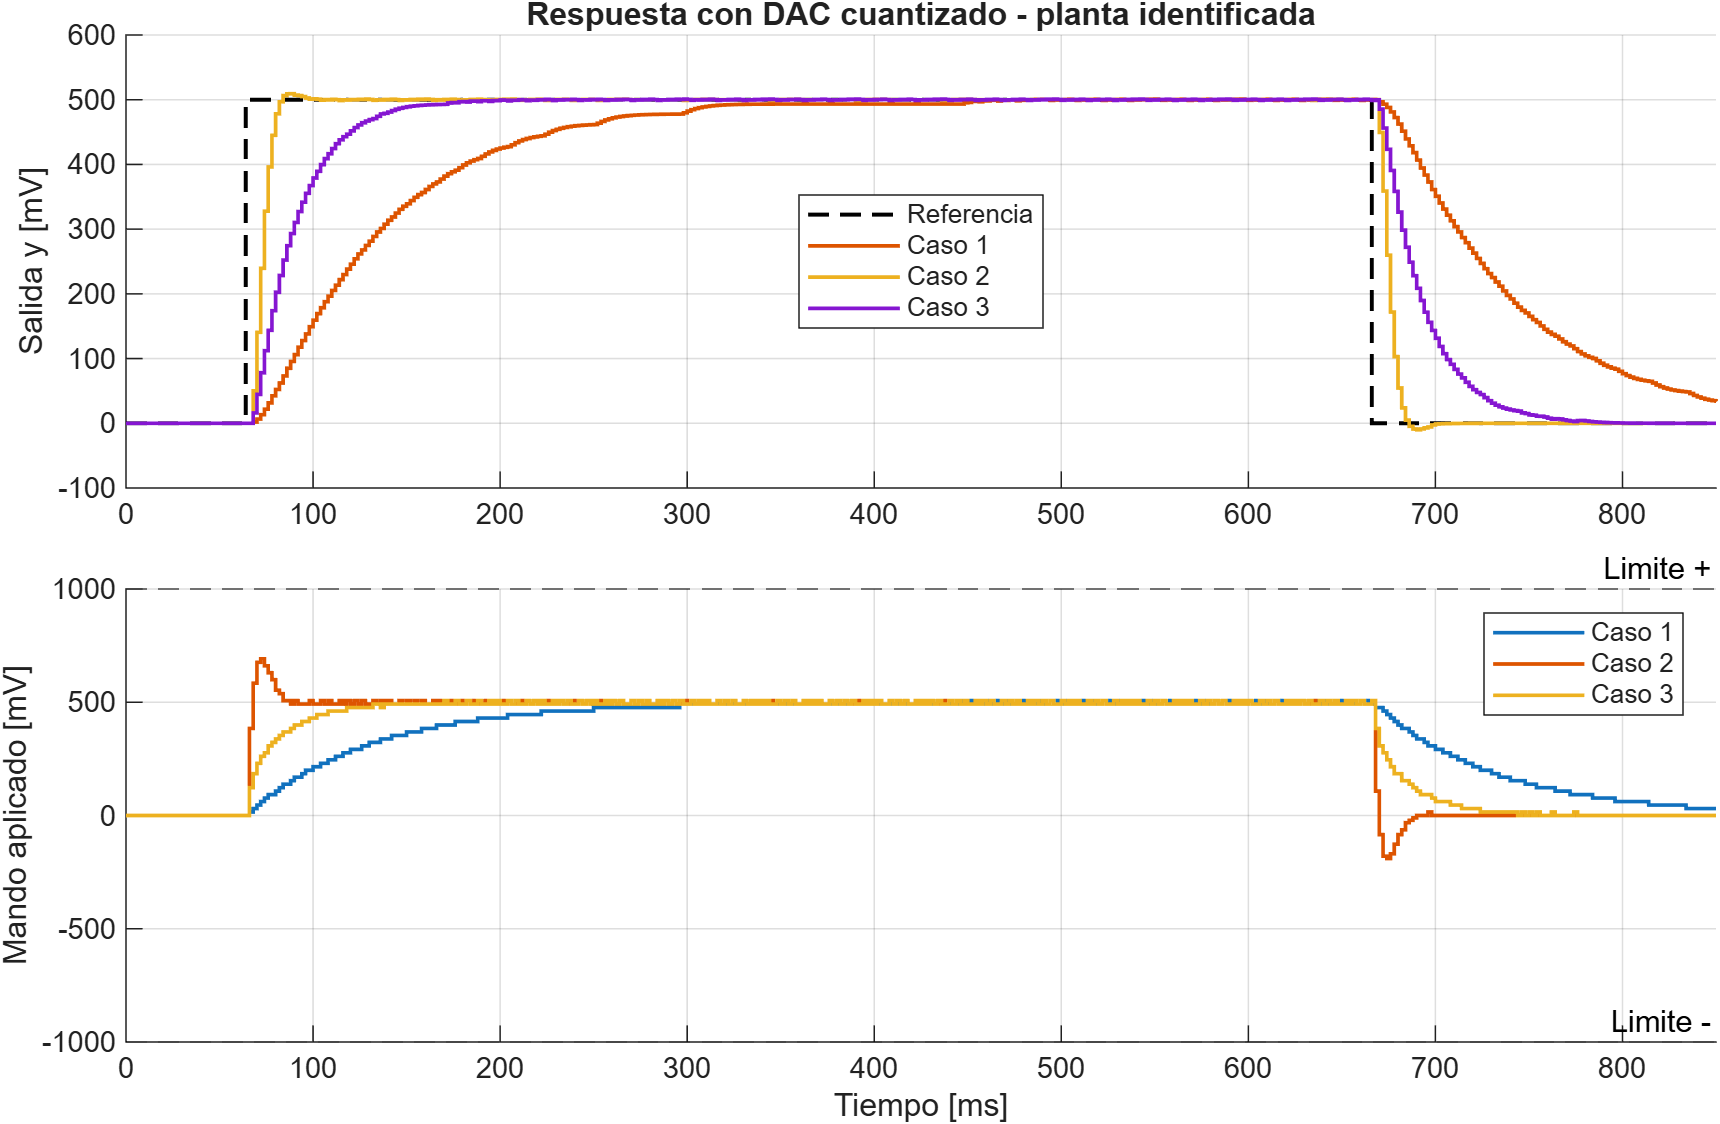
\includegraphics[width=\columnwidth]{comparacion_lqr_identificada.png}
\caption{Respuesta simulada de los tres controladores sobre el modelo identificado con DAC cuantizado.}
\label{fig:simulacion}
\end{figure}

\section{Ensayo experimental}
La programación se realizó desde PSoC Creator 4.4. Antes del cierre de lazo se aplicó un pulso abierto de \SI{0.5}{V}; J5 alcanzó \SI{0.480}{V} y J7 \SI{0.496}{V}, con lo que se verificaron signo, cableado y escala.

Para cada controlador se armó el RIGOL DS1202Z-E en modo de disparo único. CH1 se conectó a J5 para medir el mando y CH2 a J7 para medir la salida. Se usaron puntas en 1X, \SI{0.2}{V/div} en ambos canales, \SI{200}{ms/div} y límite de ancho de banda. El nivel de \SI{50}{mV} se empleó únicamente para disparar sobre CH1; la referencia aplicada fue de \SI{0.5}{V}. Cada CSV contiene 1200 muestras por canal con separación de \SI{2}{ms}. Las métricas se calcularon desde estos archivos; una media móvil de siete muestras se utilizó sólo para evitar que un código aislado modificara los cruces de umbral.

\begin{figure}[!t]
\centering
\includegraphics[width=0.92\columnwidth]{rigol_caso_2_pantalla_lab9.png}
\caption{Pantalla original del RIGOL para el caso 2. CH1 (amarillo) es el mando J5 y CH2 (cian) la salida J7; el escalón ocupa aproximadamente 2,5 divisiones verticales.}
\label{fig:rigol_original}
\end{figure}

\begin{table*}[!t]
\caption{Valores calculados, simulados y medidos para una referencia de \SI{0.5}{V}}
\label{tab:comparacion}
\centering
\scriptsize
\begin{tabular}{cclrrrrr}
\toprule
Caso & Origen & $t_r$ [ms] & $t_{s,2\%}$ [ms] & $M_p$ [\%] &
$e_{ss}$ [mV] & $u_{\min}$ [mV] & $u_{\max}$ [mV]\\
\midrule
1 & Calculado & 148 & 270 & 0,00 & 0,084 & 0 & 498\\
1 & Simulado con DAC & 148 & 248 & 0,18 & $-0,041$ & 0 & 507\\
1 & Medido & 146 & 264 & 0,98 & 15,8 & 0 & 480\\
\midrule
2 & Calculado & 12 & 18 & 1,94 & $\approx0$ & $-188$ & 687\\
2 & Simulado con DAC & 12 & 18 & 1,84 & $-0,036$ & $-190$ & 692\\
2 & Medido & 16 & 34 & 3,48 & 16,9 & $-223$ & 681\\
\midrule
3 & Calculado & 48 & 92 & 0,00 & $\approx0$ & 0 & 499\\
3 & Simulado con DAC & 48 & 90 & 0,18 & $-0,044$ & 0 & 507\\
3 & Medido & 46 & 88 & 1,81 & 20,0 & $-22$ & 482\\
\bottomrule
\end{tabular}
\end{table*}

\begin{figure*}[!b]
\centering
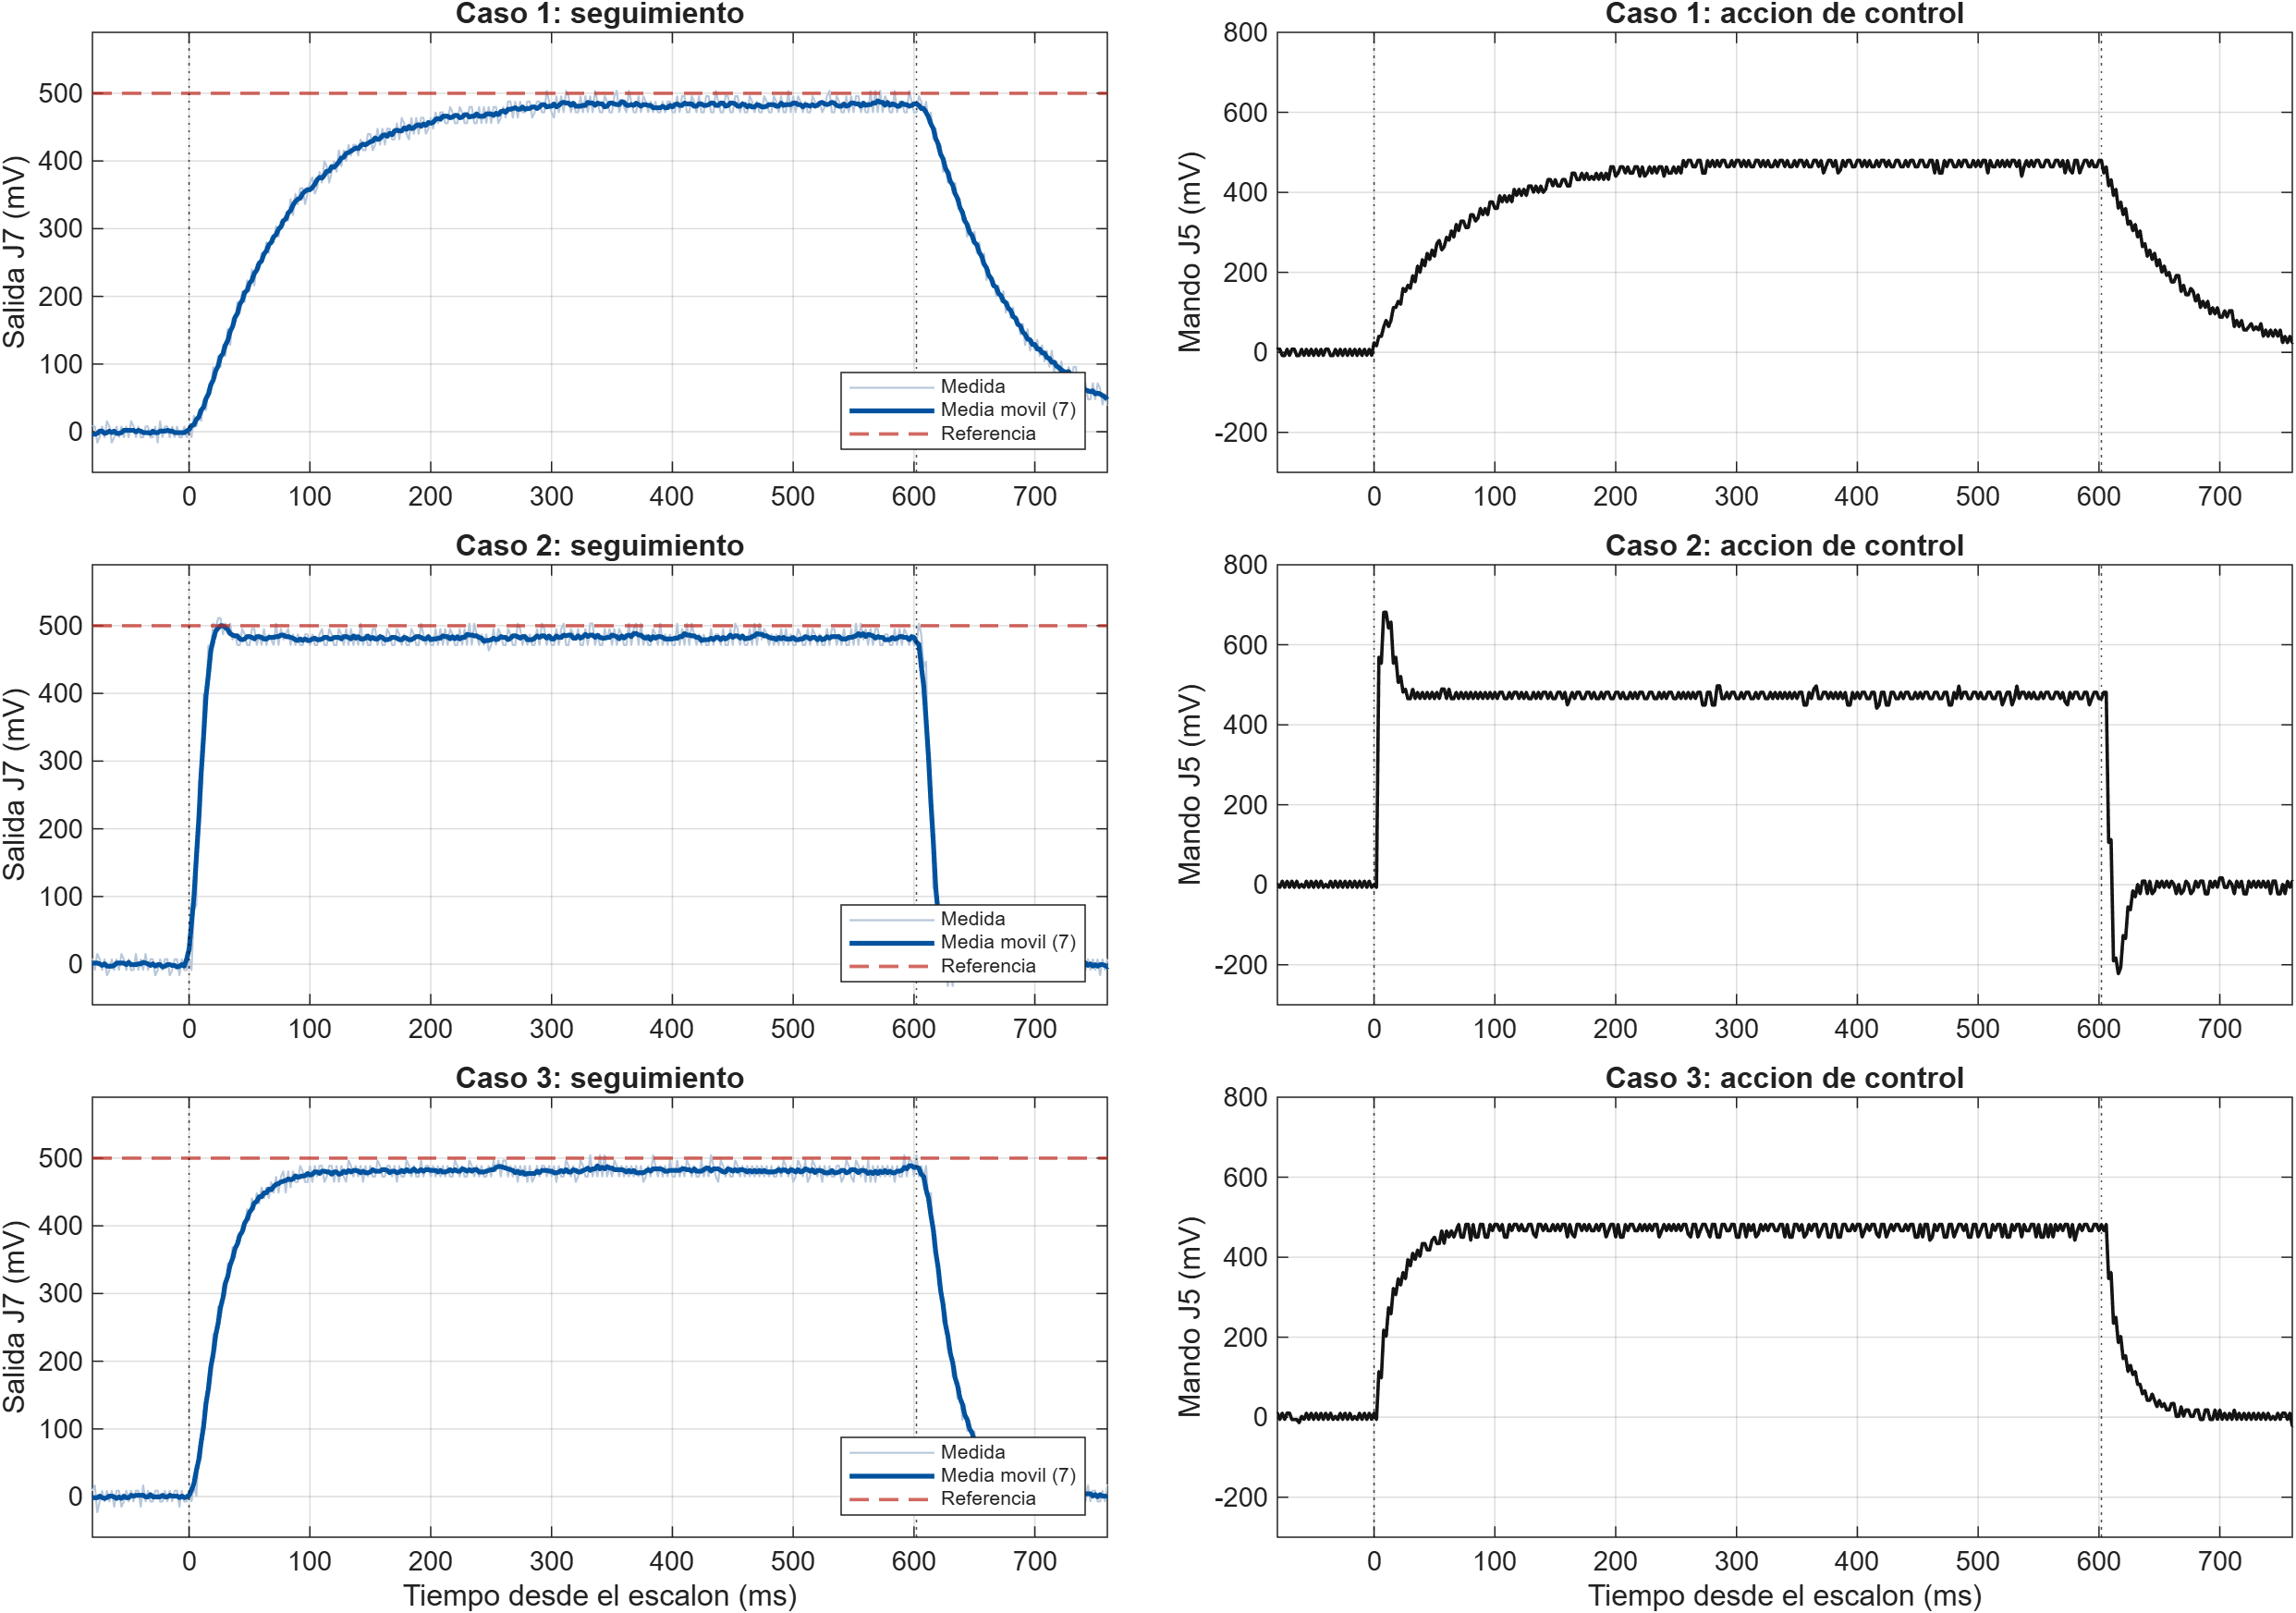
\includegraphics[width=0.92\textwidth,height=0.48\textheight,keepaspectratio]{respuesta_experimental_rigol_lab9.png}
\caption{Señales experimentales reconstruidas directamente desde los CSV del RIGOL. A la izquierda se muestran J7 y su media móvil; a la derecha, el mando físico en J5.}
\label{fig:experimental}
\end{figure*}

En el Cuadro~\ref{tab:comparacion}, ``Calculado'' corresponde al modelo identificado con actuador continuo ideal limitado y ``Simulado con DAC'' incorpora cuantización y asimetría de las ramas. Las métricas $t_r$, $t_s$ y $M_p$ se obtuvieron respecto del nivel final de cada respuesta, mientras que $e_{ss}$ se mantuvo referido a los \SI{0.5}{V}. Los residuos menores que \SI{0.1}{mV} en los modelos se deben a la ventana finita de cálculo; en esas condiciones, la acción integral lleva el error prácticamente a cero. En el montaje, en cambio, ninguna respuesta permaneció dentro de la banda de seguimiento de $\pm\SI{10}{mV}$ antes de retirar el pulso. Los errores finales equivalen a 3,16\,\%, 3,39\,\% y 4,00\,\% de la referencia.

El orden de rapidez coincidió con la predicción. Frente a la simulación con DAC, las diferencias de $t_r$ fueron $-2$, $+4$ y \SI{-2}{ms}; equivalen a una, dos y una muestras, respectivamente. Para $t_s$ las diferencias fueron $+16$, $+16$ y \SI{-2}{ms}. Por ello, el 88,9\,\% del caso 2 debe leerse junto con su diferencia absoluta de \SI{16}{ms}: el porcentaje aumenta porque el valor simulado es de apenas \SI{18}{ms}. Los casos 1 y 3 mostraron la concordancia más estrecha, mientras que el caso 2 conservó la mayor sensibilidad a dinámicas no representadas y a la resolución temporal. Su pico positivo medido de \SI{681}{mV} quedó próximo a los \SI{692}{mV} simulados y lejos del límite de \SI{1}{V}.

\section{Conclusiones}
El modelo identificado permitió construir un sistema aumentado controlable y un estimador observable. Los tres diseños fueron estables y la solución de Riccati coincidió con \texttt{dlqr} dentro de $3.35\times10^{-11}$.

El barrido de amplitud mostró que \SI{0.5}{V} es una referencia adecuada: ocupa unas 2,5 divisiones en la escala utilizada y mantiene el peor mando previsto en \SI{0.687}{V}. Las referencias de 0,75 y \SI{1}{V} no respetaron el margen adoptado y llegaron a saturar.

En el banco, los tiempos de subida de 146, 16 y \SI{46}{ms} mantuvieron el orden previsto por el diseño. Los casos 1 y 3 difirieron menos de 5\,\% de la simulación, y en el caso 2 la diferencia de 33,3\,\% corresponde a \SI{4}{ms}, es decir, dos períodos de muestreo. Este último fue el más rápido y también el más exigente, con un intervalo medido de $-223$ a \SI{681}{mV}. Los otros dos casos ofrecieron respuestas más suaves, con picos positivos de 480 y \SI{482}{mV}. Ningún controlador alcanzó el límite físico.

La diferencia principal apareció en régimen: los errores finales quedaron entre 15,8 y \SI{20.0}{mV}, por lo que no se sostuvo la banda de seguimiento del 2\,\% alrededor de la referencia. La separación explícita entre establecimiento dinámico y error estacionario evita atribuir este sesgo a una respuesta lenta. La ganancia estática real y los offsets de la cadena de medida todavía condicionan la precisión final. Aun así, el caso 2 reprodujo con buena precisión el esfuerzo máximo simulado y los tres ensayos fueron claramente visibles en el osciloscopio. Finalmente, el PSoC quedó programado en \texttt{MONITOR}, con la actuación bloqueada.

\enlargethispage{2\baselineskip}
\begin{thebibliography}{9}
\bibitem{ogata}
K. Ogata, \emph{Discrete-Time Control Systems}, 2nd ed. Prentice Hall, 1995.

\bibitem{franklin}
G. F. Franklin, J. D. Powell and M. L. Workman, \emph{Digital Control of Dynamic Systems}, 3rd ed. Addison-Wesley, 1998.
\end{thebibliography}

\AddToShipoutPictureFG{%
  \ifnum\value{page}=4
    \AtPageLowerLeft{%
      \raisebox{0.20in}{\makebox[\paperwidth][r]{\footnotesize SDG\hspace*{0.25in}}}%
    }%
  \fi
}

\end{document}
